\documentclass{report}
\usepackage[hidelinks]{hyperref}
\usepackage{amsthm}
\usepackage{amsmath}
\usepackage{amssymb}
\usepackage{amsfonts}
\usepackage{xcolor}
\usepackage{mathrsfs}
\usepackage[framemethod=tikz]{mdframed}


\theoremstyle{definition}
\newmdtheoremenv[
  hidealllines=true,
  leftline=true,
  innerleftmargin=10pt,
  innerrightmargin=10pt,
  innertopmargin=0pt,
]{remark}{Remark}
\newtheorem{note}{Note}

\theoremstyle{definition}
\newmdtheoremenv[
    hidealllines=true,
    innerleftmargin=0pt,
    innerrightmargin=0pt,
    fontcolor=red
]{errata}{Errata}
% \newtheorem{remark}{Remark}

\theoremstyle{plain}
\newtheorem{theorem}{Theorem}
\newtheorem{definition}[theorem]{Definition}
\newtheorem{lemma}[theorem]{Lemma}
\newtheorem{proposition}[theorem]{Proposition}
\newtheorem{corollary}[theorem]{Corollary}
\numberwithin{theorem}{section}
\numberwithin{remark}{section}
\numberwithin{equation}{section}
\newcommand{\norm}[1]{\lVert#1\rVert}
\newcommand{\abs}[1]{\left\lvert#1\right\rvert}
\newcommand{\absl}[1]{\lvert#1\rvert}
\renewcommand{\Re}{\operatorname{Re}}
\renewcommand{\Im}{\operatorname{Im}}
\newcommand{\sgn}{\operatorname{sgn}}
\newcommand{\sign}{\operatorname{sign}}
\newcommand{\BMO}{\operatorname{BMO}}
\newcommand{\argmax}{\operatorname{argmax}}
\newcommand{\supp}{\operatorname{supp}}
\begin{document}
\chapter{The Littlewood-Paley Theory and Multipliers}
\begin{note}
    In this book notation, the Fourier transform of $f$ is $\int f(x)e^{2\pi i t\cdot x} dx$ instead of $\int f(x)e^{-2\pi i t\cdot x} dx$. And the inverse Fourier transform in this book is $\int \hat{f}(x)e^{-2\pi i t\cdot x} dx$. But we will still use the common notation.
\end{note}
There are three main topic originally in the Littlewood-Paley theory:
\begin{enumerate}
    \item The auxiliary $g$-function
    \item Partial sum operators and the dyadic decomposition
    \item Marcinkiewicz multiplier theorem
\end{enumerate}
All these three topics are related to multipliers. The auxiliary $g$-function helps us prove Mihlin multiplier theorem (section 3) and further some multipliers in $M_p$ for specific $p$. Partial sum operator (section 4) shows some indicate functions of convex sets are multipliers. Also with help of partial sum operator, we can prove Marcinkiewicz multiplier theorem (section 6). This theorem and Mihlin multiplier theorem overlap and neither includes the other.
\section{The first tool: The Littlewood-Paley $g$-function}
For a function $f\in L^p(\mathbb{R}^n)$, we define its Poisson integral is:
\begin{equation*}
    u(x,y)=\int_{\mathbb{R}^n}P_y(t)f(x-t)d t
\end{equation*}
where $P_y(t)=\int_{\mathbb{R}^n}e^{-2\pi\abs{x}y}e^{-2\pi i t\cdot x }dx=\frac{c_ny}{(\abs{t}^2+y^2)^{\frac{n+1}{2}}}$. The $g$-function of $f$ is:
\begin{equation*}
    g(f)(x)=\left( \int_{0}^{\infty} \abs{\nabla u(x,y)}^2 y d y\right)^\frac{1}{2}
\end{equation*}
One application of $g$-function is it can control the norm of $f$:
\begin{theorem}\label{thm: g-function control f}
    Suppose $f\in L^p(\mathbb{R}^n)$, $1<p<\infty$. Then $g(f)\in L^p(\mathbb{R}^n)$ and
    \begin{equation*}
        A'_p\norm{f}_p\leq \norm{g(f)}_p\leq A_p\norm{f}_p
    \end{equation*}
\end{theorem}
For $p=2$, we have identity $\norm{g(f)}_2= 2^{-\frac{1}{2}}\norm{f}_2$. This identity is important in dyadic decomposition.\par
The part $\norm{g(f)}_p\leq A_p\norm{f}_p$ is from vector-valued analogues of singular integral. \par
Define
\begin{equation*}
    \mathscr{H}_2^0=\left\{ f: \abs{f}^2=\int_{0}^{\infty}\abs{f(y)}^2y dy<\infty \right\}
\end{equation*}
and $\mathscr{H}_2$ be the direct sum of n+1 copies of $\mathscr{H}_2^0$.\par
The kernel of singular integral here is $K_\epsilon(x)=(\frac{\partial P_{y+\epsilon(x)}}{\partial y},\frac{\partial P_{y+\epsilon(x)}}{\partial x_1},\dots,\frac{\partial P_{y+\epsilon(x)}}{\partial x_k})$. Notice $\abs{\nabla u(x,y+\epsilon)}^2\leq \abs{\nabla u(x,y)}^2$. We have $\abs{T_\epsilon(f)(x)}=\abs{\int_{\mathbb{R}^n}{K_\epsilon(t)f(x-t)dt}}\leq g(f)(x)$ ($T_\epsilon(f)(x)$ is in Hilbert space) and $T_\epsilon(f)(x)$ converges to $g(f)(x)$ pointwise.\par
The converse part $ A'_p\norm{f}_p\leq \norm{g(f)}_p$ is by polarization to the identity, Holder inequality and dual of $L^p$.
\section{The function $g_{\lambda}^*$}
First section is relied on singular integral. In this section we give the same result based on characteristic properties of harmonic functions. The ideas here are useful when singular integral is not applicable.\par
Author shows how to avoid singular integral method to prove the following inequality
\begin{equation}\label{ieq: first control}
    \norm{g(f)}_p\leq A_p\norm{f}_p\quad (1<p\leq 2)
\end{equation}
The case $2<p<\infty$ is not shown here.\par
In the rest of this section, we talk about the positive function $g_{\lambda}^*$
\begin{equation*}
    (g_{\lambda}^*(f)(x))^2=\int_{0}^{\infty}\int_{t\in \mathbb{R}^n}{(\frac{y}{\abs{t}+y})^{\lambda n}\abs{\nabla u(x-t,y)}^2 y^{1-n}dt dy}
\end{equation*}
The first important inequality is:
\begin{equation}
    g(f)(x)\leq CS(f)(x)\leq C_\lambda g_{\lambda}^*(f)(x)
\end{equation}
where 
\begin{equation*}
    (S(f)(x))^2=\int_{\Gamma(x)}{\abs{\nabla u(t,y)}^2 y^{1-n}dydt}=\int_{\Gamma}{\abs{\nabla u(x-t,y)}^2 y^{1-n}dydt}
\end{equation*}
where $\Gamma=\left\{ (t,y)\in \mathbb{R}_+^{n+1}: \abs{t}<y, y>0\right\}$ and $\Gamma(x)$ is cone $\Gamma$ with vertex at $x$.\par
The second important inequality is:
\begin{equation}
    \norm{g_{\lambda}^*(f)(x)}_p\leq A_{p,\lambda}\norm{f}_p\quad (1<p<\infty, p>\frac{2}{\lambda}).   
\end{equation}\par
The case $p\geq 2$ is by proving $\norm{g_{\lambda}^*(f)}_p\leq A_\lambda\norm{g(f)}_p$ and inequality \eqref{ieq: first control}. It is interesting that the p-norm of $g(f)$, $g_{\lambda}^*(f)$ can control each other when $p\geq 2$.\par
The proof for the case $p<2$ is like the proof for inequality \eqref{ieq: first control}.\par
We conclude that the norm of $g_{\lambda}^*(f)$, $g(f)$, $S(f)$, $f$ can control each other.
\section{Multipliers (first version)}
Most of results in this section can be found in section 6, chapter 2 in Rubio's \emph{Weighted Norm inequalities and Related topics}. And proofs of results are in my note of that book.\par
Multiplier $m$ is related to a linear transformation $T_m$ defined as:
\begin{equation*}
    (T_mf)^\wedge(x)=m(x)\hat{f}(x)
\end{equation*}
and we shall say that $m$ is a multiplier for $L^p$ if:
\begin{equation*}
    \norm{T_mf}_p\leq \norm{f}_p
\end{equation*}\par
Multipliers has some general properties:
\begin{enumerate}
    \item $M_p$ is a Banach algebra under pointwise multiplication.
    \item $M_2$ is identical with the bounded measurable function $L^\infty$.
    \item $M_1$ is identical with the finite Borel measures $\mathscr{B}$ (Refer Theorem 2.5.8 in \emph{Classical Fourier Analysis}).
    \item Suppose $\frac{1}{p}+\frac{1}{q}=1$, $1\leq p,q\leq \infty$, then $M_p=M_q$ with identity of norms.
    \item $M_\infty$ is identical with the finite Borel measures $\mathscr{B}$ (By 3 and 4).
\end{enumerate}
Then we prove two important multiplier theorems. The first is Mihlin multiplier theorem:
\begin{theorem}
    Suppose that $m(x)$ is of class $C^k$ in the complement of the origin of $\mathbb{R}^n$, where $k$ is an integer greater than $\frac{n}{2}$. Assume also that for every differential monomial $(\frac{\partial}{\partial x})^\alpha$, $\alpha=(\alpha_1,\alpha_2,\dots,\alpha_n)$, with $\abs{\alpha}=\alpha_1+\alpha_2+\cdots+\alpha_n$, we have:
    \begin{equation}\label{ieq: Mihlin}
        \abs{\frac{\partial}{\partial x}^\alpha m(x)}\leq B\abs{x}^{-\abs{\alpha}},\quad \abs{\alpha}\leq k
    \end{equation}
    Then $m\in M_p$, $1<p<\infty$
\end{theorem}
And the second is H\"{o}rmander Mihlin multiplier theorem:
\begin{theorem}
    The assumption \eqref{ieq: Mihlin} can be replaced by the weaker assumptions:
    \begin{equation*}
        \abs{m(x)}\leq B
    \end{equation*}
    \begin{equation*}
        \sup_{0<R<\infty}R^{2\abs{\alpha}+n}\int_{R\leq\abs{x}\leq 2R}{\abs{\frac{\partial}{\partial x}^\alpha m(x)}^2 dx}\leq B,\quad \abs{\alpha}\leq k
    \end{equation*}
\end{theorem}
The proof of Mihlin multiplier theorem can be done with help of g-functions and their variants:
\begin{lemma}
    Under the assumption \eqref{ieq: Mihlin}, let us set for each $f\in L^2$:
    \begin{equation*}
        F(x)=(T_mf)(x)
    \end{equation*}
    Then
    \begin{equation*}
        g_1(F,x)\leq B_\lambda g_\lambda^*(f,x),\quad \lambda=\frac{2k}{n}
    \end{equation*}
\end{lemma}
By above lemma, we have:
\begin{equation*}
    \norm{T_mf}_p=\norm{F}_p\leq A_1\norm{g_1(F,x)}_p\leq A_2\norm{g_\lambda^*(f,x)}_p\leq A_3\norm{f}_p
\end{equation*}
{\color{blue}I can not understand the proof of corollary in the end of this section.}\par
\section{The second tool: partial sums operators}
Given a rectangle $\rho$, we define he partial sum operator $S_\rho(f)$ to be:
\begin{equation*}
    S_\rho(f)^\wedge=\chi_\rho\hat{f}
\end{equation*}
and for this operator we have:
\begin{equation}\label{ieq: partial sum operator inequality}
    \norm{S_\rho(f)}_p\leq A_p\norm{f}_p\quad 1<p<\infty
\end{equation}
This bounded linear operator has an extended version on function space $L^p(\mathbb{R}^n,\mathscr{H})$, where $\mathscr{H}$ is the sequence Hilbert space: $\mathscr{H}=\{(c_j)_{j=1}^\infty:(\sum_j\abs{c_j}^2)^\frac{1}{2}< \infty\}$.\par
Given a sequence of rectangle $\mathscr{R}=\{\rho_j\}_{j=1}^\infty$, we define
\begin{equation*}
    S_{\mathscr{R}}(f)=(S_{\rho_1}(f_1),\dots,S_{\rho_j}(f_j),\dots)
\end{equation*}
where
\begin{equation*}
    f=(f_1,\dots,f_j,\dots)
\end{equation*}\par
The general version of inequality \eqref{ieq: partial sum operator inequality} is
\begin{equation}\label{ieq: partial sum operator inequality 2}
    \norm{S_{\mathscr{R}}(f)}_p\leq A_p\norm{f}_p\quad 1<p<\infty
\end{equation}\par
To prove this theorem, we use vector-valued analogues of Hilbert transform. But first we consider the one dimensional and single valued case. We have following identity for operator $S_{(-\infty,0)}$:
\begin{equation}\label{eq: Hilbert for -infty to 0}
    S_{(-\infty,0)}=\frac{I+iH}{2}
\end{equation}
For one dimensional and vector-valued case, by property of vector-valued singular integral, we have:
\begin{equation*}
    \norm{\tilde{H}f}_p\leq A_p\norm{f}_p
\end{equation*}
where $\tilde{H}f=(Hf_1,\dots,Hf_j,\dots)$. Combining with equation \eqref{eq: Hilbert for -infty to 0}, we have inequality \eqref{ieq: partial sum operator inequality 2} holds when $f$ is vector-valued with single variable and $\mathscr{R}$ is collection of rectangles $(-\infty,0)$.\par
By translation, we can show:
\begin{equation*}
    S_{(-\infty,a_j)}f_j(x)=\frac{f_j+ie^{2\pi i x\cdot a_j}H(e^{-2\pi i x\cdot a_j}f_j)}{2}
\end{equation*}
Thus inequality \eqref{ieq: partial sum operator inequality 2} holds when $f$ is vector-valued with single variable and $\mathscr{R}$ is collection of rectangles $(-\infty,a_j)$.\par
To prove n dimensional case, we claim:
\begin{lemma}[Linear span is dense in section 4.2.3]
    The linear span of form $f'(x_1)f''(x_2,\dots,x_n)$ is dense in $L^2(\mathbb{R}^n)$.
\end{lemma}
This lemma is true since we can choose $f'$ and $f''$ as orthogonal basis of $L^2(\mathbb{R})$ and $L^2(\mathbb{R}^{n-1})$. By this lemma, we can consider first variable $x_1$ separately. Thus inequality \eqref{ieq: partial sum operator inequality 2} holds when $f$ is vector-valued with n variables and $\mathscr{R}$ is collection of half space $\{x:x_1<a_j\}_{j=1}^\infty$.\par
Finally since finite rectangle is the intersection of 2n half-spaces, a 2n-fold of previous result proves the inequality \eqref{ieq: partial sum operator inequality 2} where $\mathscr{R}$ contains finite rectangles. The result is not depended on number of rectangles. Thus using limit argument the inequality \eqref{ieq: partial sum operator inequality 2} holds for infinite number of rectangles.\par
The author describes two problems:
\begin{enumerate}
    \item Let $B$ be the unit ball in $\mathbb{R}^n$. Can we replace the rectangle $\rho$ by the ball $B$ in inequality \eqref{ieq: partial sum operator inequality}?.
    \item Can the rectangles of inequality \eqref{ieq: partial sum operator inequality 2} be replaced by rectangles that are each arbitrarily rotated?
\end{enumerate}
We know the the answer of first problems can be affirmative only in the range $\frac{2n}{n+1}<p<\frac{2n}{n-1}$. The solution of first problem implies the resolution of the second problem for the same $p$. And the answer of the second problem is in the negative for $p$ outside the interval $\frac{2n}{n+1}\leq p\leq \frac{2n}{n-1}$.\par
Also there is a continuous analogue of inequality \eqref{ieq: partial sum operator inequality 2}. Let $(\Gamma,d\gamma)$ be an abstract measure space. We can replace the sequence Hilbert space by square integrable functions space $L^2(\Gamma,d\gamma)$. And $\rho_\gamma=\rho(\gamma)$ is a measurable function from $\Gamma$ to rectangles in $\mathbb{R}^n$.\par
\section{The dyadic decomposition}
First we introduce the dyadic decomposition of $\mathbb{R}$. We decompose $\mathbb{R}\setminus \{0\}$ as $(\cup_{k=\infty}^\infty [2^k,2^{k+1}])\cup(\cup_{k=\infty}^\infty [-2^{k+1},-2^k])$. Then we consider the product of intervals in decomposition of $\mathbb{R}$. This is the dyadic decomposition of $\mathbb{R}^n$ and we denote as $\Delta$.\par
Recall the partial sum operator, we have:
\begin{equation*}
    \sum_{\rho\in \Delta}S_{\rho}=I
\end{equation*}
and since the rectangles in decomposition are disjoint, by Plancherel's theorem we have:
\begin{equation}\label{eq: decomposition 2-norm}
    \sum_{\rho\in \Delta}\norm{S_{\rho}f}_2^2=\norm{f}_2^2
\end{equation}
The special property of partial sum operator on dyadic decomposition is we can control the norm of $f$ by this partial sum operator:
\begin{theorem}\label{thm: dyadic decomposition}
    Suppose $f\in L^p$, $1<p<\infty$. Then $\left( \sum_{\rho\in \Delta}\abs{S_{\rho}f(x)}^2 \right)^\frac{1}{2}\in L^p$ and
    \begin{equation*}
        A_p\norm{f}_p\leq \norm{( \sum_{\rho\in \Delta}\abs{S_{\rho}f(x)}^2)^\frac{1}{2}}_p\leq B_p\norm{f}_p
    \end{equation*}
\end{theorem}
To prove above theorem we need Rademacher functions $\{r_i(t)\}_{i=1}$ on integral $(0,1)$. $r_0(t)$ is defined to be:
\begin{equation*}
    r_0(t)=
    \left\{\begin{aligned}
        1\quad 0<t\leq \frac{1}{2}\\
        -1\quad \frac{1}{2}\leq t< 1
    \end{aligned}\right.
\end{equation*} 
and $r_m(t)$ is defined to be $r_0(2^mt)$ and they are extended outside by periodicity. The important of Rademacher functions is all p-norms of linear combination of Rademacher functions are comparable:
\begin{theorem}
    Suppose $\sum\abs{a_m}^2<\infty$ and set $F(t)=\sum a_mr_m(t)$. Then $F(t)\in L^p$ for all $p<\infty$ and
\begin{equation*}
    A_p\norm{F}_p\leq\norm{F}_2=\left( \sum_{m=0}^\infty\abs{a_m}^2 \right)^{\frac{1}{2}}\leq B_p\norm{F}_p
\end{equation*}
\end{theorem}
By equation \eqref{eq: decomposition 2-norm}, we only need to proof one inequality in theorem \ref{thm: dyadic decomposition}:
\begin{equation*}
    \norm{( \sum_{\rho\in \Delta}\abs{S_{\rho}f(x)}^2)^\frac{1}{2}}_p\leq B_p\norm{f}_p
\end{equation*}
The other inequality is by polarization and dual of $L^p$.
\section{The Marcinkiewicz multiplier theorem}
The Marcinkiewicz multiplier theorem is one of the most important results of the Littlewood-Paley theory
\begin{theorem}
    Let $m$ be a bounded function on $\mathbb{R}^n$ of the type described. Suppose also
    \begin{enumerate}
        \item $\abs{m}\leq B$
        \item for each $0<k\leq n$
        \begin{equation*}
            \sup_{x_{k+1},\dots,x_n}\int_{\rho}\abs{\frac{\partial^km}{\partial x_1\dots\partial x_k}}dx_1\dots dx_k\leq B
        \end{equation*}
        \item The condition analogous to 2. is valid for every on of the $n!$ permutations of the variables $x_1,\dots,x_n$.
    \end{enumerate}
    Then $m\in M_p$, $1<p<\infty$; and more precisely, if $f\in L^2\cap L^p$, $\norm{T_mf}_p\leq A_p\norm{f}_p$ where $A_p$ depends only on $B$, $p$ and $n$.
\end{theorem}
The difference between H\"ormander multiplier theorem and Marcinkiewicz multiplier theorem can be illustrated by invariance considerations. The class of multipliers in H\"omander multiplier theorem is invariant under dilations, $m(x)\mapsto m(\epsilon x)$ and rotations $m(x)\mapsto m(\rho^{-1} x)$. But the class of multipliers in Marcinkiewicz multiplier theorem is invariant under a larger group of dilations, $m(x)\mapsto m(\epsilon\circ x)$, where $\epsilon\circ x=(\epsilon_1x_1,\dots,\epsilon_nx_n)$. But it not invariant under rotations.\par
Let $\Delta$ denote the dyadic decomposition and $f\in L^2\cap L^p$, and write $F=T_mf$. To prove this theorem, we only need to show:
\begin{equation*}
    \norm{(\sum_{\rho\in \Delta}\abs{S_\rho F}^2)^\frac{1}{2}}_p\leq C_p\norm{(\sum_{\rho\in \Delta}\abs{S_\rho f}^2)^\frac{1}{2}}_p
\end{equation*}
Using Theorem \ref{thm: dyadic decomposition} we conclude $m\in M_p$.
\section{Details of proof and errata, section 1}
\begin{note}[section 1.2]
    We have identity:
    \begin{equation*}
        u(x,y)=\int_{\mathbb{R}^n}\hat{f}(t)e^{2\pi it\cdot x}e^{-2\pi \abs{t}y}d t
    \end{equation*}
    Then:
    \begin{equation*}
        \frac{\partial u}{\partial y}=\int_{\mathbb{R}^n}-2\pi\abs{t}\hat{f}(t)e^{2\pi it\cdot x}e^{-2\pi \abs{t}y}d t
    \end{equation*}
    and
    \begin{equation*}
        \frac{\partial u}{\partial x_j}=\int_{\mathbb{R}^n}2\pi i{t_j}\hat{f}(t)e^{2\pi it\cdot x}e^{-2\pi \abs{t}y}d t
    \end{equation*}
    Notice $(\frac{\partial u}{\partial y})^\wedge=-2\pi\abs{t}\hat{f}(t)e^{-2\pi \abs{t}y}$ and $(\frac{\partial u}{\partial x_j})^\wedge=2\pi i{t_j}\hat{f}(t)e^{-2\pi \abs{t}y}$. Thus by Plancherel's theorem:
    \begin{align*}
        \int_{\mathbb{R}^n}{\abs{\nabla u(x,y)}^2 dx}= & \int_{\mathbb{R}^n}\abs{\frac{\partial u}{\partial y}}^2 dx+\sum_{j=1}^n\int_{\mathbb{R}^n}\abs{\frac{\partial u}{\partial x_j}}^2 dx                   \\
        =                                              & \int_{\mathbb{R}^n}\abs{(\frac{\partial u}{\partial y})^\wedge}^2 d t+\sum_{j=1}^n\int_{\mathbb{R}^n}\abs{(\frac{\partial u}{\partial x_j})^\wedge}^2 d t \\
        =                                              & \int_{\mathbb{R}^n} 4\pi^2(\abs{t}^2+\sum_{j=1}^n \abs{t_j}^2) \absl{\hat{f(t)}}^2 e^{-4\pi\abs{t}y} d t                                                 \\
        =                                              & \int_{\mathbb{R}^n} 8\pi^2\abs{t}^2\absl{\hat{f(t)}}^2 e^{-4\pi\abs{t}y} d t
    \end{align*}
\end{note}
\begin{errata}[P83]
    Missing $d y$ in bracket:
    \begin{equation*}
        \int_{\mathbb{R}^n}\absl{\hat{f}(t)}^2\left\{ 8\pi^2\abs{t}^2\int_{0}^{\infty}e^{-4\pi\abs{t}y}y d y\right\}d t
    \end{equation*}
\end{errata}
\begin{note}[section 1.3]
    We have following estimations:
    \begin{equation*}
        \frac{\partial P_y}{\partial y}=\frac{c_n}{(\abs{x}^2+y^2)^{\frac{n+1}{2}}}+\frac{2c_ny^2}{(\abs{x}^2+y^2)^{\frac{n+3}{2}}}\leq \frac{c_n}{(\abs{x}^2+y^2)^{\frac{n+1}{2}}}+\frac{2c_n(\abs{x}^2+y^2)}{(\abs{x}^2+y^2)^{\frac{n+3}{2}}}\leq \frac{A}{(\abs{x}^2+y^2)^{\frac{n+1}{2}}}
    \end{equation*}
    \begin{equation*}
        \frac{\partial^2 P_y}{\partial y\partial x_j}=\frac{2c_n\abs{x_j}}{(\abs{x}^2+y^2)^{\frac{n+3}{2}}}+\frac{4c_ny^2\abs{x_j}}{(\abs{x}^2+y^2)^{\frac{n+5}{2}}}\leq \frac{A\abs{x_j}}{(\abs{x}^2+y^2)^{\frac{n+3}{2}}}
    \end{equation*}
    \begin{equation*}
        \frac{\partial P_y}{\partial x_i}=\frac{2c_ny\abs{x_i}}{(\abs{x}^2+y^2)^{\frac{n+3}{2}}} \leq \frac{c_n(y^2+\abs{x_i}^2)}{(\abs{x}^2+y^2)^{\frac{n+3}{2}}} \leq\frac{A}{(\abs{x}^2+y^2)^{\frac{n+1}{2}}}
    \end{equation*}
    \begin{equation*}
        \frac{\partial^2 P_y}{\partial x_i\partial x_j}=\frac{4c_ny\abs{x_i}\abs{x_j}}{(\abs{x}^2+y^2)^{\frac{n+5}{2}}} \leq\frac{A\abs{x_j}}{(\abs{x}^2+y^2)^{\frac{n+3}{2}}}\quad (i\neq j)
    \end{equation*}
    \begin{equation*}
        \frac{\partial^2 P_y}{\partial x_i^2}=\frac{\pm 2c_ny}{(\abs{x}^2+y^2)^{\frac{n+3}{2}}}+\frac{4c_ny\abs{x_i}\abs{x_j}^2}{(\abs{x}^2+y^2)^{\frac{n+5}{2}}} \leq\frac{A(\abs{x_j}+y)}{(\abs{x}^2+y^2)^{\frac{n+3}{2}}}
    \end{equation*}
    Thus
    \begin{equation*}
        \abs{\frac{\partial K_{\epsilon}(x)}{\partial x_j}}^2\leq \frac{A\abs{x_j}^2}{(\abs{x}^2+y^2)^{{n+3}}}+\frac{(n-1)A\abs{x_j}^2}{(\abs{x}^2+y^2)^{{n+3}}}+\frac{A(\abs{x_j}+y)^2}{(\abs{x}^2+y^2)^{{n+3}}}\leq \frac{A}{(\abs{x}^2+y^2)^{{n+2}}}
    \end{equation*}
\end{note}
\begin{note}[section 1.4]
    \begin{theorem}[Polarization to the identity]
        \begin{equation*}
            <x,y>=\frac{1}{4}\sum_{k=0}^3 i^k\norm{x+i^ky}^2
        \end{equation*}
    \end{theorem}
Notice $g_1(f)$ is not an linear map. Denote $u(f)(x)=\int_{\mathbb{R}^n}{P_y(t)f(x-t)d t}$. Using the fact that $\mathscr{H}_2^0$ is a Hilbert space:
\begin{align*}
    \int_{\mathbb{R}^n}{f_1\bar{f_2}}=&<f_1,f_2>=\frac{1}{4}\sum_{k=0}^3 i^k\norm{f_1+i^kf_2}_2^2=\sum_{k=0}^3 i^k\norm{g_1(f_1+i^kf_2)}_2^2\\
    =&\int_{\mathbb{R}^n}{(\sum_{k=0}^3 \int_0^{\infty}i^k\abs{\frac{\partial u(f_1+i^kf_2)}{\partial y}}^2 y d y )}dx\\
    =&\int_{\mathbb{R}^n}{(\sum_{k=0}^3 i^k\int_0^{\infty}\abs{\frac{\partial u(f_1)}{\partial y}+i^k\frac{\partial u(f_2)}{\partial y}}^2 y d y  )}dx\\
    =&4\int_{\mathbb{R}^n}{\int_0^{\infty}{\frac{\partial u(f_1)}{\partial y}\overline{\frac{\partial u(f_2)}{\partial y}}} y d y  }dx
\end{align*}
Using Holder inequality:
\begin{align*}
    \abs{\int_{\mathbb{R}^n}{f_1\bar{f_2}}}\leq& 4\int_{\mathbb{R}^n}{\int_0^{\infty}\abs{\frac{\partial u(f_1)}{\partial y}\overline{\frac{\partial u(f_2)}{\partial y}}} y d y  }dx\\
    \leq& 4\int_{\mathbb{R}^n} \left(\int_0^{\infty}    \abs{\frac{\partial u(f_1)}{\partial y}}^2y d y  \right)^\frac{1}{2} \left(\int_0^{\infty}   \abs{\frac{\partial u(f_2)}{\partial y}}^2y d y  \right)^\frac{1}{2} dx\\
    \leq& 4\int_{\mathbb{R}^n} g_1(f_1)(x) g_1(f_2)(x) dx
\end{align*}
\end{note}
\begin{errata}[P85]
    \begin{equation*}
        \abs{\int_{\mathbb{R}^n}{f_1\bar{f_2}}}    \leq 4\int_{\mathbb{R}^n} g_1(f_1)(x) g_1(f_2)(x) dx
    \end{equation*}
    % \begin{equation*}
    %     \abs{\int_{\mathbb{R}^n}{f_1\bar{f_2}}}    \leq 4\norm{g_1(f_1)}_p\norm{g_1(f_2)}_q \leq 4A_q\norm{g_1(f_1)}_p\norm{f_2}_q
    % \end{equation*}
\end{errata}
\begin{note}[section 1.5]
    \begin{align*}
        (g_k(f,x))^2=&\int_{0}^{\infty}\abs{\frac{\partial^{k}u(x,y)}{\partial y^{k}}}^2y^{2k-1}d y\\
        \leq&\int_{0}^{\infty}\left( \int_{y}^{\infty}\abs{\frac{\partial^{k+1}u(x,s)}{\partial s^{k+1}}}^2s^{2k}ds\left( \int_{y}^{\infty}s^{-2k}ds \right) \right) y^{2k-1}d y\\
        =&\frac{1}{2k-1}\int_{0}^{\infty}\left( \int_{y}^{\infty}\abs{\frac{\partial^{k+1}u(x,s)}{\partial s^{k+1}}}^2s^{2k}ds ~y^{-2k+1} \right) y^{2k-1}d y\\
        =&\frac{1}{2k-1}\int_{0}^{\infty} \int_{y}^{\infty}\abs{\frac{\partial^{k+1}u(x,s)}{\partial s^{k+1}}}^2s^{2k}ds d y\\
        =&\frac{1}{2k-1}\int_{0}^{\infty} \int_{0}^{s}\abs{\frac{\partial^{k+1}u(x,s)}{\partial s^{k+1}}}^2s^{2k}d y ds\\
        =&\frac{1}{2k-1}\int_{0}^{\infty} \abs{\frac{\partial^{k+1}u(x,s)}{\partial s^{k+1}}}^2s^{2k+1} ds\\
        =&(g_{k+1}(f,x))^2
    \end{align*}    
\end{note}
\begin{errata}[P86]
    Lower index of $\int_{y}^{\infty}s^{-2k}ds$ is $y$ instead of $1$.
    \begin{equation*}
        \int_{y}^{\infty}\abs{\frac{\partial^{k+1}u(x,s)}{\partial s^{k+1}}}^2s^{2k}ds\left( \int_{y}^{\infty}s^{-2k}ds \right)
    \end{equation*}
\end{errata}
\section{Details of proof and errata, section 2}
\begin{note}[Lemma 1 in section 2.1]
    The $\Delta$ is applied on $u^p$. Since $\frac{\partial^2 u^p}{\partial x_i^2}=p((p-1)u^{p-2}(\frac{\partial u}{\partial x_i})^2+u^{p-1}\frac{\partial^2 u}{\partial x_i^2})$ and $u$ is harmonic, we have $\Delta(u^p)=p((p-1)u^{p-2}\abs{\nabla u}^2+u^{p-1}\Delta u)=p(p-1)u^{p-2}\abs{\nabla u}^2$.
\end{note}
\begin{errata}[P89]
In equation (18) is $\int_{\Gamma}{\abs{\Delta u(x-t,y)}^2 y^{1-n}d y d t}$
\end{errata}
\begin{note}[$g(f)(x)\leq CS(f)(x)$ in section 2.3]
    Recall:
    \begin{equation*}
        g(f)(x)=\left( \int_{0}^{\infty} \abs{\nabla u(x,y)}^2 y d y\right)^\frac{1}{2}
    \end{equation*}
    and
    \begin{equation*}
        (S(f)(x))^2=\int_{\Gamma(x)}{\abs{\nabla u(t,y)}^2 y^{1-n}dydt}=\int_{\Gamma}{\abs{\nabla u(x-t,y)}^2 y^{1-n}dydt}
    \end{equation*}
The proof here using mean-value theorem. Thus we only need to prove the case $x=0$. The general case is proved by moving the center of ball $B_y$ to $x$.\par
From figure \ref{fig1}, it is clear that $(x,s)\in B_y$ implies $s\in ((1-\frac{1}{\sqrt{2}})y,(1+\frac{1}{\sqrt{2}})y)$. Thus $y\in ((\frac{\sqrt{2}}{\sqrt{2}+1})s,(\frac{\sqrt{2}}{\sqrt{2}-1})s)$. The inequality at the end of page 90 is by $y$ and $s$ controlling each other.
\begin{figure}[h!]
    \centering
    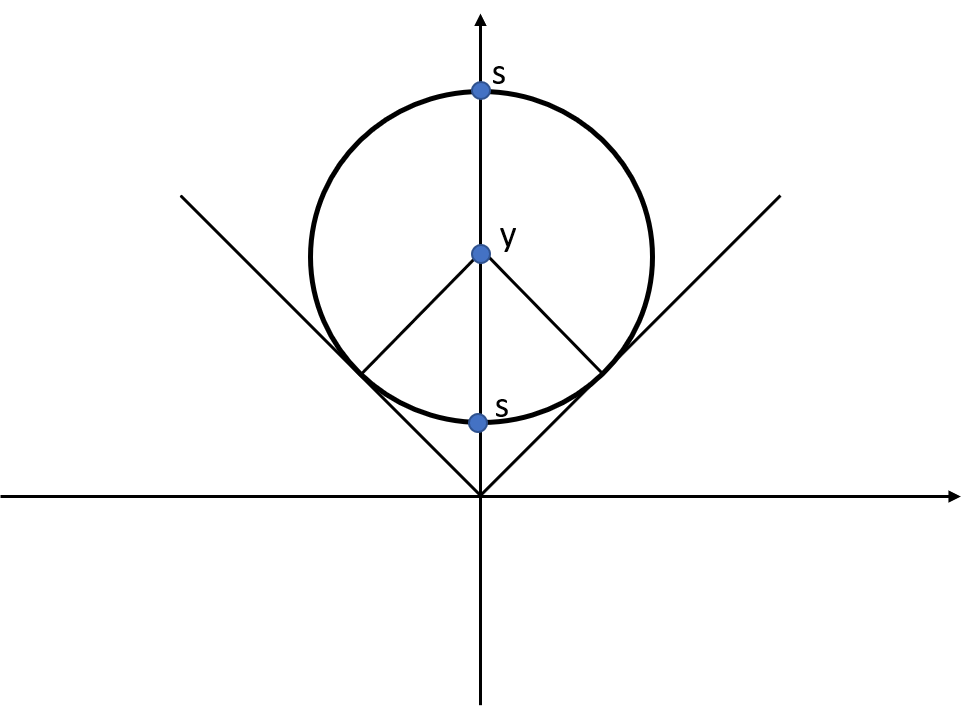
\includegraphics[width = 0.7\textwidth]{Picture1.png}
    \caption{Ball $B_y$ and s}
    \label{fig1}
\end{figure}
\end{note}
\begin{note}[Proof of theorem 2 in section 2.4]
    $\lambda>1$ guarantees that for $\phi(x)=(1+\abs{x})^{-\lambda n}$, $(\phi_\epsilon(x))$ are approximations to the identity. \par
\end{note}
\begin{note}[Proof in section 2.5]
    Since Poisson kernel is homogeneous of degree -n, the convolution $P*f$ is homogeneous of degree 0.\par
    $Q_t(x)\leq c_n$ for $\abs{x}\leq 2\abs{t}$ and $Q_t(x)\leq A'(1+\abs{x}^2)^{\frac{-n-1}{2}}$ for $\abs{x}> 2\abs{t}$. Thus:
    \begin{align*}
        \int_{\mathbb{R}^n}Q_t(x)dx=&\int_{\abs{x}\leq 2\abs{t}}Q_t(x)dx+\int_{\abs{x}\leq 2\abs{t}}Q_t(x)dx\\
        \leq&\int_{\abs{x}\leq 2\abs{t}}c_n dx+\int_{\abs{x}\leq 2\abs{t}}A'(1+\abs{x}^2)^{\frac{-n-1}{2}}dx\\
        \leq&\int_{0}^{2\abs{t}}c_n r^{n-1} dr+\int_{2\abs{t}}^{\infty} A'(1+r^2)^{\frac{-n-1}{2}}r^{n-1}dr\\
        \leq&\frac{c_n2^n}{n}\abs{t}^{n} +\int_{0}^{\infty} A'(1+r^2)^{\frac{-n-1}{2}}r^{n-1}dr\\
        \leq&\frac{c_n2^n}{n}\abs{t}^{n} +\int_{0}^{\frac{\pi}{2}} A'(\sin{u})^{n-1}du\\
        \leq&\frac{c_n2^n}{n}\abs{t}^{n} +C\\
        \leq&A(1+\abs{t})^n\\
    \end{align*}\par
    Estimation for $\int_{\mathbb{R}^n}{\frac{dx}{(1+\abs{x})^{\lambda'n}}}$
    \begin{align*}
        \int_{\mathbb{R}^n}{\frac{dx}{(1+\abs{x})^{\lambda'n}}}=&C\int_{0}^{\infty}\frac{r^{n-1}dr}{(1+r)^{\lambda'n}}\\
        =&C\int_{1}^{\infty}\frac{(r-1)^{n-1}dr}{r^{\lambda'n}}\\
        \leq&C\int_{1}^{\infty}\frac{1}{r^{\lambda'n}}C_1\sum_{k=0}^{n-1}r^k dr\\
        \leq&C\sum_{k=0}^{n-1}\int_{1}^{\infty}r^{k-\lambda'n} dr\\
        \leq&C\sum_{k=0}^{n-1}\frac{1}{k-\lambda'n+1}\\
        <&\infty
    \end{align*}
\end{note}
\section{Details of proof and errata, section 3}
\begin{note}[proof in section 3.3.1]
    Inequality (34) does not need hypothesis (30).\par
    By Leibniz's rule:
    \begin{align*}
            \abs{(\frac{\partial}{\partial x})^\alpha (\abs{x}^km(x))}\leq& C\sum_{\alpha=\beta+\gamma}\abs{(\frac{\partial}{\partial x})^\beta\abs{x}^k}\abs{(\frac{\partial}{\partial x})^\gamma m(x)}\\
            \leq &C\sum_{\alpha=\beta+\gamma} (\abs{x}^{k-2\abs{\beta}}\prod_{\beta}\abs{x_j}^{\beta_j})B\abs{x}^{-\abs{\gamma}}\\
            \leq &C\sum_{\alpha=\beta+\gamma} (\abs{x}^{k-\abs{\beta}})B\abs{x}^{-\abs{\gamma}}\\
            \leq &B'\abs{x}^{k-\abs{\alpha}}
    \end{align*}
    To estimate $\abs{(\frac{\partial}{\partial x})^\alpha (\abs{x}^km(x)e^{-2\pi\abs{x}y})}$, we need following:
    \begin{align*}
        \abs{(\frac{\partial}{\partial x_i}) e^{-2\pi\abs{x}y}}=2\pi y e^{-2\pi\abs{x}y}\frac{\abs{x_i}}{\abs{x}}
    \end{align*} 
    \begin{align*}
        \abs{(\frac{\partial^2}{\partial x_ix_j}) e^{-2\pi\abs{x}y}}=&2\pi y (\frac{\partial}{\partial x_j})(e^{-2\pi\abs{x}y}\frac{\abs{x_i}}{\abs{x}})\\
        \leq&2\pi y\left(  (\frac{\partial}{\partial x_j})e^{-2\pi\abs{x}y} \right)\frac{\abs{x_i}}{\abs{x}}+2\pi ye^{-2\pi\abs{x}y}\left((\frac{\partial}{\partial x_j})\frac{\abs{x_i}}{\abs{x}}\right)\\
        \leq&4\pi^2 y^2 e^{-2\pi\abs{x}y} \frac{\abs{x_ix_j}}{\abs{x}^2}+2\pi ye^{-2\pi\abs{x}y}\frac{\abs{x_ix_j}}{\abs{x}^3}
    \end{align*} 
    
    Thus by induction:

    \begin{align*}
        \abs{(\frac{\partial}{\partial x})^\gamma e^{-2\pi\abs{x}y}}\leq&e^{-2\pi\abs{x}y}\sum_{k=1}^{\abs{\gamma}}(2\pi y)^k\frac{\abs{x^\gamma}}{\abs{x}^{2\abs{\gamma}-k}}\\
        \leq&e^{-2\pi\abs{x}y}\sum_{k=1}^{\abs{\gamma}}(2\pi y)^k\abs{x}^{k-\abs{\gamma}}\\
        \leq&\frac{e^{-2\pi\abs{x}y}}{\abs{x}^{\abs{\gamma}}}\sum_{k=1}^{\abs{\gamma}}(2\pi y)^k\abs{x}^{k}\\
    \end{align*} 
    So we have following estimation:
    \begin{align*}
        &\abs{(\frac{\partial}{\partial x})^\alpha (\abs{x}^km(x)e^{-2\pi\abs{x}y})}\\
        \leq & C\sum_{\alpha=\beta+\gamma}\abs{(\frac{\partial}{\partial x})^\beta\abs{x}^km(x)}\abs{(\frac{\partial}{\partial x})^\gamma e^{-2\pi\abs{x}y}}\\
        \leq & C\sum_{\alpha=\beta+\gamma}B'\abs{x}^{k-\abs{\beta}}\frac{e^{-2\pi\abs{x}y}}{\abs{x}^{\abs{\gamma}}}\sum_{l=1}^{\abs{\gamma}}(2\pi y)^l\abs{x}^{l}\\
        \leq & C\sum_{\alpha=\beta+\gamma}B'\abs{x}^{k-\abs{\alpha}}{e^{-2\pi\abs{x}y}}\sum_{l=1}^{\abs{\gamma}}(2\pi y)^l\abs{x}^{l}\\
        \leq & C'\abs{x}^{k-\abs{\alpha}}{e^{-2\pi\abs{x}y}}\sum_{\alpha=\beta+\gamma}\sum_{l=1}^{\abs{\gamma}}(2\pi y)^l\abs{x}^{l}\\
    \end{align*}
Let $k=\alpha$ and use inequality in book, we have:
\begin{align*}
    &\int_{\mathbb{R}^n}\abs{(\frac{\partial}{\partial x})^\alpha (\abs{x}^km(x)e^{-2\pi\abs{x}y})}^2 dx\\
    \leq & C'\sum_{r=1}^{m}\int_{\mathbb{R}^n}(2\pi y)^r\abs{x}^{r}e^{-4\pi\abs{x}y}dx\\
    \leq & C'\sum_{r=1}^{m}Cy^{-n}\\
\end{align*}
where $m$ is a finite value. Thus $\int_{\mathbb{R}^n}\abs{(\frac{\partial}{\partial x})^\alpha (\abs{x}^km(x)e^{-2\pi\abs{x}y})}^2 dx\leq B'y^{-n}$.
\end{note}
\begin{note}[proof in section 3.3.2]
    \begin{align*}
        \abs{U^{(k+1)(x,y)}}^2=&\left( \int_{\mathbb{R}^n}{M^{(k)}(t,\frac{y}{2})u^{(1)}(x-t,\frac{y}{2})dt} \right)^2\\
        \leq &\left( \int_{\abs{t}\leq\frac{y}{2}}{M^{(k)}(t,\frac{y}{2})u^{(1)}(x-t,\frac{y}{2})dt} \right)^2+\left( \int_{\abs{t}>\frac{y}{2}}{M^{(k)}(t,\frac{y}{2})u^{(1)}(x-t,\frac{y}{2})dt} \right)^2\\
        \leq &\left( \int_{\abs{t}\leq\frac{y}{2}}{\abs{M^{(k)}(t,\frac{y}{2})}^2dt} \right) \left( \int_{\abs{t}\leq\frac{y}{2}}{\abs{u^{(1)}(x-t,\frac{y}{2})}^2dt} \right)\\
         &+\left( \int_{\abs{t}>\frac{y}{2}}{\abs{t}^{2k}\abs{M^{(k)}(t,\frac{y}{2})}^2dt} \right)\left( \int_{\abs{t}>\frac{y}{2}}\frac{\abs{u^{(1)}(x-t,\frac{y}{2})}^2dt}{\abs{t}^{2k}} \right)\\
         \leq &\left( \int_{\abs{t}\leq\frac{y}{2}}{B'y^{-2n-2k}dt} \right) \left( \int_{\abs{t}\leq\frac{y}{2}}{\abs{u^{(1)}(x-t,\frac{y}{2})}^2dt} \right)\\
         &+B'y^{-n} \left( \int_{\abs{t}>\frac{y}{2}}\frac{\abs{u^{(1)}(x-t,\frac{y}{2})}^2dt}{\abs{t}^{2k}} \right)\\
         \leq & B'y^{-2n-2k} y^{n}  \int_{\abs{t}\leq\frac{y}{2}}{\abs{u^{(1)}(x-t,\frac{y}{2})}^2dt} +B'y^{-n}  \int_{\abs{t}>\frac{y}{2}}\frac{\abs{u^{(1)}(x-t,\frac{y}{2})}^2dt}{\abs{t}^{2k}} \\
         \leq & B'y^{-n-2k} \int_{\abs{t}\leq\frac{y}{2}}{\abs{u^{(1)}(x-t,\frac{y}{2})}^2dt}+B'y^{-n} \int_{\abs{t}>\frac{y}{2}}\frac{\abs{u^{(1)}(x-t,\frac{y}{2})}^2dt}{\abs{t}^{2k}} \\
    \end{align*}
\end{note}

% \begin{note}[proof of the corollary]
%     Inequality $\abs{M^{(k)}(x,y)}\leq B'y^{-n-k}$ still holds. But 
%     by Leibniz's rule:
%     \begin{align*}
%             \abs{(\frac{\partial}{\partial x})^\alpha (\abs{x}^km(x))}\leq& C\sum_{\alpha=\beta+\gamma}\abs{(\frac{\partial}{\partial x})^\beta\abs{x}^k}\abs{(\frac{\partial}{\partial x})^\gamma m(x)}\\
%             \leq &C\sum_{\alpha=\beta+\gamma} (\abs{x}^{k-2\abs{\beta}}\prod_{\beta}\abs{x_j}^{\beta_j})\abs{(\frac{\partial}{\partial x})^\gamma m(x)}\\
%             \leq &C\sum_{\alpha=\beta+\gamma} (\abs{x}^{k-\abs{\beta}})\abs{(\frac{\partial}{\partial x})^\gamma m(x)}\\
%     \end{align*}
%     So we have following estimation:
%     \begin{align*}
%         &\abs{(\frac{\partial}{\partial x})^\alpha (\abs{x}^km(x)e^{-2\pi\abs{x}y})}\\
%         \leq & C\sum_{\alpha=\beta+\gamma}\abs{(\frac{\partial}{\partial x})^\beta\abs{x}^km(x)}\abs{(\frac{\partial}{\partial x})^\gamma e^{-2\pi\abs{x}y}}\\
%         \leq & C\sum_{\alpha=\beta+\gamma} \left(\sum_{\beta=\beta_1+\beta_2} (\abs{x}^{k-\abs{\beta_1}}) \abs{(\frac{\partial}{\partial x})^{\beta_2} m(x)}\right) \frac{e^{-2\pi\abs{x}y}}{\abs{x}^{\abs{\gamma}}}\sum_{l=1}^{\abs{\gamma}}(2\pi y)^l\abs{x}^{l}\\
%         \leq & C\sum_{\alpha=\beta+\gamma}B'\abs{x}^{k-\abs{\alpha}}{e^{-2\pi\abs{x}y}}\sum_{l=1}^{\abs{\gamma}}(2\pi y)^l\abs{x}^{l}\\
%         \leq & C'\abs{x}^{k-\abs{\alpha}}{e^{-2\pi\abs{x}y}}\sum_{\alpha=\beta+\gamma}\sum_{l=1}^{\abs{\gamma}}(2\pi y)^l\abs{x}^{l}\\
%     \end{align*}
% \end{note}
\section{Details of proof and errata, section 4 and 5}

\begin{note}[Dual in section 5.3.1]
    \begin{align*}
        \int f\bar{g}dx=&<f,g>=\frac{1}{4}\sum_{k=0}^3 i^k\norm{f+i^kg}_2^2=\frac{1}{4}\sum_{k=0}^3 i^k\sum_{\rho\in \Delta}\norm{S_\rho(f+i^kg)}_2^2\\
        =&\frac{1}{4}\sum_{k=0}^3 i^k\sum_{\rho\in \Delta}\norm{S_\rho(f)+i^kS_{\rho}(g)}_2^2=\frac{1}{4}\sum_{\rho\in \Delta}\sum_{k=0}^3 i^k\norm{S_\rho(f)+i^kS_{\rho}(g)}_2^2\\
        =&\sum_{\rho\in \Delta} \int S_\rho(f)\overline{S_{\rho}(g)}dx\\
    \end{align*}
\end{note}
\begin{note}[equation (50)]
    Assume $\abs{\phi'(x)}\leq B$. Since $\phi'_{I_m}(x)=2^{-m}\phi'(2^{-m}x)$ and $x\in [2^m,2^{m+1}]$, we have:
\begin{equation*}
    \abs{\phi'_{I_m}(x)}=2^{-m}\abs{\phi'(2^{-m}x)}\leq \frac{B}{\abs{x}}
\end{equation*}
When $I=[-2^{m+1},-2^m]$ the inequality also holds.
\end{note}
\begin{note}[inequality (53)]
    You can refer the proof in section 6.1.3 in \emph{Classical Fourier Analysis}.\par
        % By Theorem 4' in book, we have:
    % \begin{equation*}
    %     \norm{\sum_{m'}S_{I_{m'}}(\sum_m\abs{\tilde{S}_{I_m}(f)}^2)^\frac{1}{2}}_p\leq \norm{(\sum_m\abs{\tilde{S}_{I_m}(f)}^2)^\frac{1}{2}}_p
    % \end{equation*}
   Since $S_I\tilde{S}_I=S_I$, we have:
    \begin{equation*}
        \norm{( \sum_m\absl{{S}_{I_m}(f)}^2 )^\frac{1}{2}}_p=\norm{( \sum_m\absl{S_{I_m}\tilde{S}_{I_m}(f)}^2 )^\frac{1}{2}}_p
    \end{equation*}
    We want to prove:
    \begin{equation*}
        \norm{( \sum_m\absl{S_{I_m}\tilde{S}_{I_m}(f)}^2 )^\frac{1}{2}}_p\leq \norm{( \sum_m\absl{\tilde{S}_{I_m}(f)}^2 )^\frac{1}{2}}_p
    \end{equation*}
    Let $F$ be:
    \begin{equation*}
        F=(\tilde{S}_{I_1}(f),\tilde{S}_{I_2}(f),\tilde{S}_{I_3}(f),\dots)
    \end{equation*}
    So 
    \begin{equation*}
        \abs{F}=(\sum_m\abs{\tilde{S}_{I_m}(f)}^2)^\frac{1}{2}    
    \end{equation*}
    Let $\mathscr{R}$ be $\Delta_1$, we have
    \begin{equation*}
        S_{\mathscr{R}}(F)=(S_{I_1}\tilde{S}_{I_1}(f),S_{I_2}\tilde{S}_{I_2}(f),S_{I_3}\tilde{S}_{I_3}(f),\dots)
    \end{equation*}
    By Theorem 4' in book, we have:
    \begin{equation*}
        \norm{( \sum_m\absl{S_{I_m}\tilde{S}_{I_m}(f)}^2 )^\frac{1}{2}}_p=\norm{S_{\mathscr{R}}(F)}_p\leq \norm{F}_p=\norm{( \sum_m\absl{\tilde{S}_{I_m}(f)}^2 )^\frac{1}{2}}_p
    \end{equation*}
\end{note}
\begin{note}[inequality (54)]
    By (46)
    \begin{equation*}
        B_p\norm{T_t^Nf}_p\leq\norm{(\sum_\rho \abs{S_\rho (T_t^Nf)}^2)^\frac{1}{2}}_p
    \end{equation*}
    Notice $S_{I_m}S_{I_m}f=S_{I_m}f$ and $S_{I_m}S_{I_n}f=0$ if $n\neq m$, we have:
    \begin{equation*}
        \sum_\rho \abs{S_\rho (T_t^Nf)}^2= \sum_{m=0}^N \abs{r_m(t)S_{I_m}f}^2\leq\sum_{m=0}^N \abs{S_{I_m}f}^2
    \end{equation*}
    Thus
    \begin{equation*}
        B_p\norm{T_t^Nf}_p\leq\norm{(\sum_\rho \abs{S_\rho (T_t^Nf)}^2)^\frac{1}{2}}_p\leq\norm{(\sum_{m=0}^N \abs{S_{I_m}f}^2)^\frac{1}{2}}_p\leq C_p\norm{f}_p
    \end{equation*}
\end{note}
\end{document}